\documentclass{article}
\usepackage{fancyhdr}
\usepackage{extramarks}
\usepackage{amsmath}
\usepackage{amsthm}
\usepackage{amsfonts}
\usepackage{tikz}
\usepackage[plain]{algorithm}
\usepackage{algpseudocode}

\begin{document}
\author{Chuan Lu}
\title{PHYS:5905 Homework 5}
\maketitle

\medskip

\begin{enumerate}
\item
Small-Angle Collision Scattering Routine

\begin{enumerate}
\item $\sigma(\theta) = \frac{\pi}{18}.$ Figure \ref{1-1}.

\begin{figure}[h]
\centering
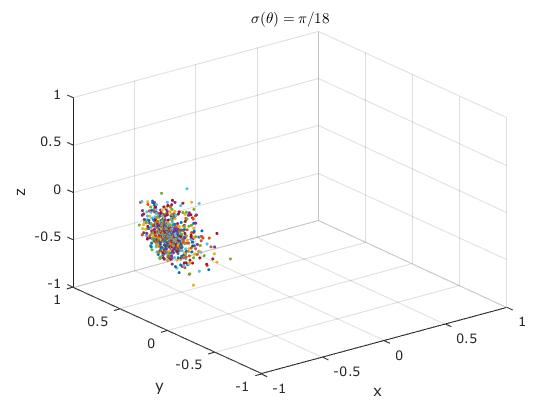
\includegraphics[scale=0.4]{problem1/pi_18.jpg}.
\label{1-1}
\caption{$\sigma(\theta) = \frac{\pi}{18}.$}
\end{figure}

\item $\sigma(\theta) = \frac{\pi}{180}$. Figure \ref{1-2}.

\begin{figure}[h]
\centering
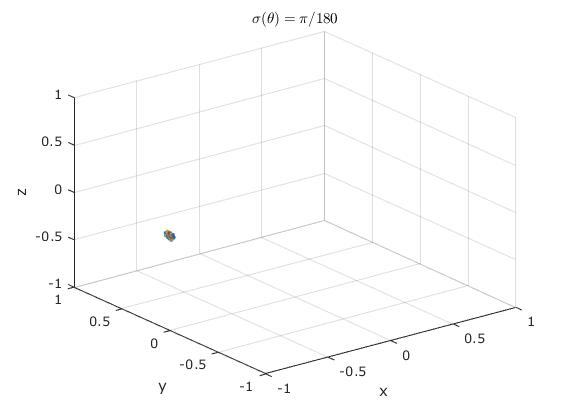
\includegraphics[scale=0.4]{problem1/pi_180.jpg}. 
\label{1-2}
\caption{$\sigma(\theta) = \frac{\pi}{180}.$}
\end{figure}

\end{enumerate}

\item
Monte Carlo Collisions

\begin{enumerate}
\item confinement time $\tau$. Figure \ref{2-1}.

\begin{figure}[h]
\centering
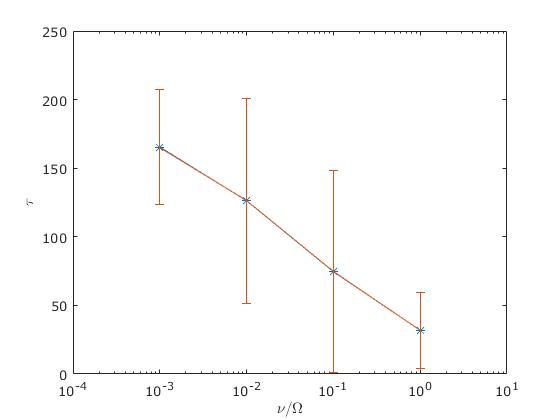
\includegraphics[scale=0.4]{problem2/confinement_time.jpg}.
\label{2-1}
\caption{mean and stand deviation of $\tau$.}
\end{figure}

\item plot of $v$. Figure \ref{2-2}.

\begin{figure}[h]
\centering
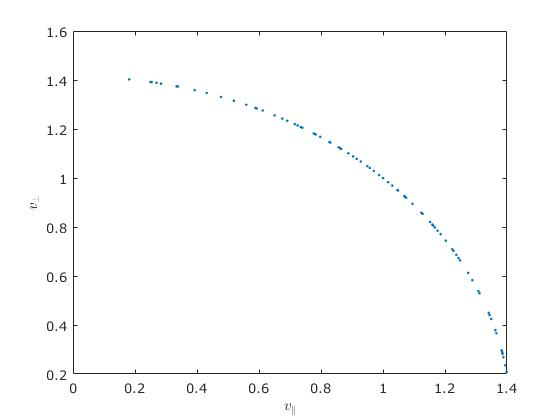
\includegraphics[scale=0.4]{problem2/v.jpg}.
\label{2-2}
\caption{position of particle in $(v_\parallel, v_\perp)$ space when the particle is lost.}
\end{figure}

\end{enumerate}

\end{enumerate}


\end{document}